\documentclass[10pt,a4paper]{article}
\usepackage[utf8]{inputenc}
\usepackage{graphicx}
\usepackage{listings}

\author{Kim Rostgaard Christensen}
\title{Information-oriented verification and validation}


\begin{document}
\maketitle

\abstract{With the increasing complexity, the need for a formalized approach to verification and validation becomes apparent to document activities, and make them traceable.}

\tableofcontents
\newpage

\section{Introduction}
This report used the EN-50126 standard for railways as the formal process to implement. As the EN-50126 contains a very general approach to V\&V, the methods discussed here could be applied more generally.

When unified Modelling Language (UML) is discussed in this report. Version 1 of UML is implied, although the latest version is 2.0.
\subsection{Background}
I noted that the QA challenges faced during the development process of a larger software project, and the QA challenges faced when producing V\&V documentation were quite similar.
%TODO


\subsection{Terminology}
The terminologies within a safety management process is largely company-culture dependant. In this report we will use the term issue describing a non-conformity with a given requirement. Whenever a requirement, or sub-requirement is anything else than conformant - it is considered an issue.

\subsubsection{Hazard log}
The hazard log is where all identified hazards go. Once identified, they go through the life cycle illustrated in figure \ref{fig:hazard_log_life_cycle}

\begin{figure}[h]
\centering
%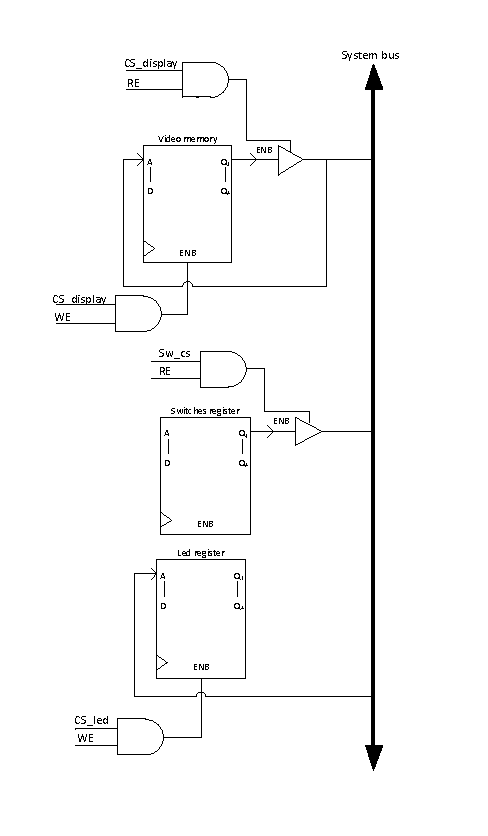
\epsfig{file=fig/system.eps, width=3.0in}
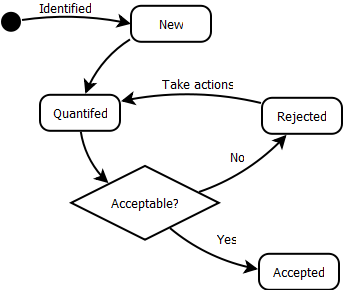
\includegraphics[scale=0.45]{fig/Hazard_log_Entry_Lifecycle.png} 
\caption{Life cycle hazard log entry}
\label{fig:hazard_log_life_cycle}
\end{figure}

\subsubsection{Traceabilty}
Traceabilty is one of the cornerstones of safety management. Each change and decision or must be tracked during the life-cycle of the entire project. This requirement is typically solved by ad-hoc document naming procedures, and similar manual procedures.

\subsection{Terminology of software project management}
Typically you have a hierarchy consisting of projects, subprojects and components. The structure is illustrated in figure \ref{fig:project_structure}.

\begin{figure}[h]
\centering
%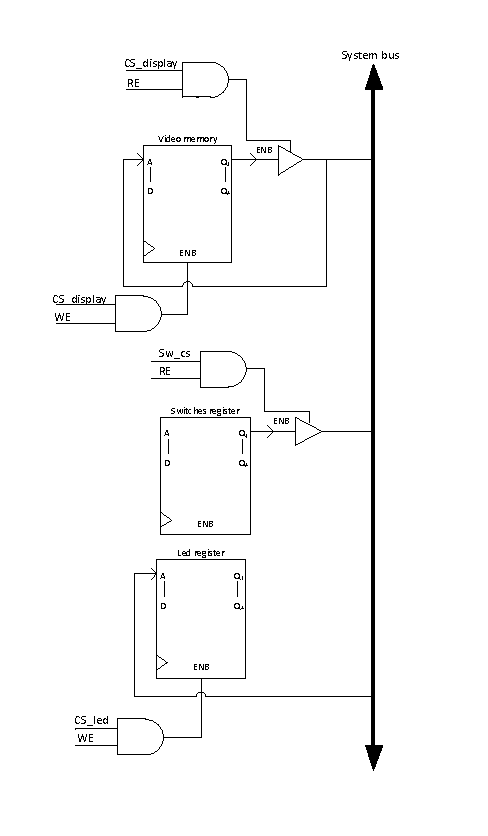
\epsfig{file=fig/system.eps, width=3.0in}
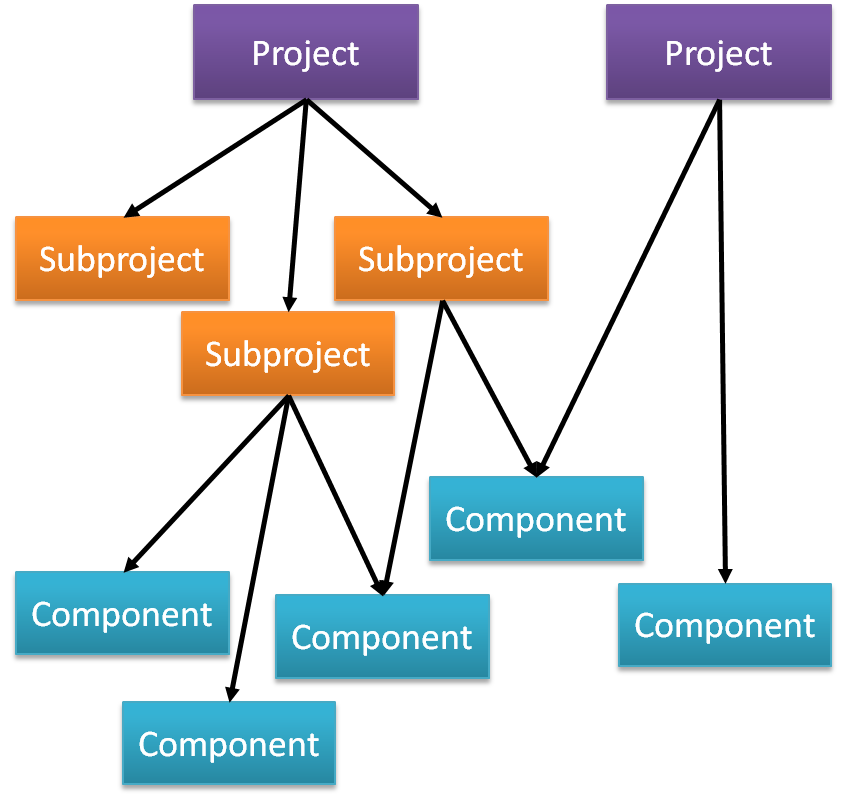
\includegraphics[scale=0.6]{fig/project_structure.png} 
\caption{Software project structure}
\label{fig:project_structure}
\end{figure}

TODO: The need for 


\subsubsection{Issues}
Issue tracking is one the critical functionalities of the tool. Figure \ref{fig:software_issue_life_cycle} illustrates the process of eliminating a software bug in a software system (a bug is ambiguous to an issue) from identification to resolution.


\begin{figure}[h]
\centering
%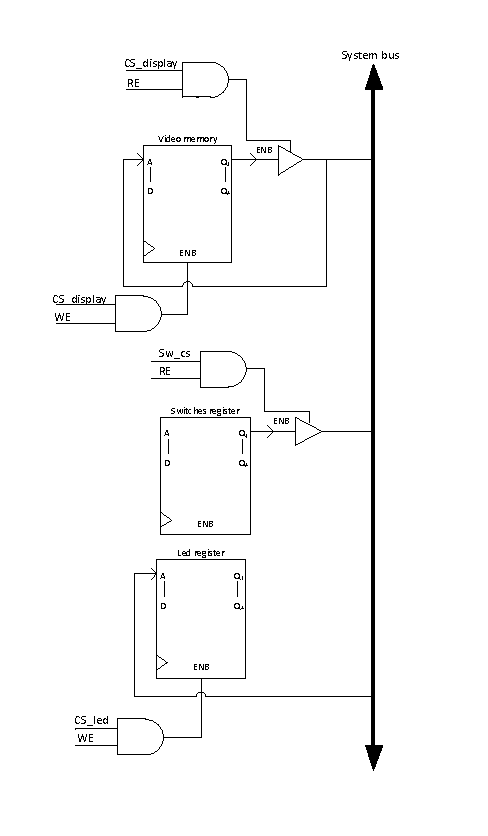
\epsfig{file=fig/system.eps, width=3.0in}
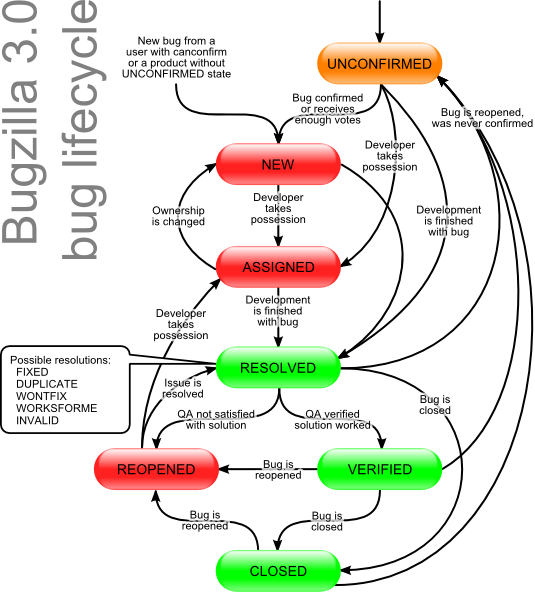
\includegraphics[scale=0.45]{fig/Bugzilla_Lifecycle_color-aqua.png} 
\caption{Life cycle of a software issue}
\label{fig:software_issue_life_cycle}
\end{figure}


\section{Mapping}
Freezing 

\section{Discussion}
The main motivation and goal for using a tool in the V\&V process must be to eliminate tedious low-practical tasks, and unify the parts of the validation process that allows it.

The tasks can include an automatic header generator filling out the revision log with the information provided by the validator.

What it is not:
It is not a strict system that decides what format your document must be written in. It is meant as a service to keep track of the tedious information - mainly traceabilty.
\section{Events}
\subsection{Quality assurance}

\subsection{Validation}
A validation starts by appointing a validator. This is done by any document author.

The validator will then receive access to the validation view of the document management system.


\section{Notes}


\subsection{Working on a shared interface document}
The following figure illustrates the differences between a classic approach and a centralized tool approach, using the process of merging two V\&V documents from two different stakeholders, with a common interface, as an example.
For the classic approach, a deadline decides when the merge will take place. In the centralized approach, a continuous merge will take place during the QS of the document. This will also have the advantage that FBAS will be able to provide comments mid-process.

\subsection{Continuous releases}
Having a shared interface for for solving issues within a document could potentially increase the work flow and overall efficiency of a QA or V\&V process. 

When an issue is marked as resolved a message will go out to every other person involved. They can, if the change is uploaded, pull down the new version of the document and verify that the issues is truly resolved. There is no need to wait for a new global revision of the document.

This is roughly corresponding to the "release often" philosophy widely, and successfully, applied in large and complex software projects.

\subsubsection{Maintaining focus}
In order to ensure an acceptable level of open issues, a number of pre-release deadlines must be defined for each deadline. All issues opened after this point, below a specified threshold (e.g. below critical), will not be taken into consideration. The purpose of these small iterations is to provide a continuously stable document throughout the life-cycle of the document.

\subsection{Personnel competencies}
EN 50126 requires a V\&V team to account for the competencies of the personnel carrying out the V\&V process. Theses qualifications could be stored within each user profile, which should be able to import from existing CV databases such as Linkedin\footnote{http://linkedin.com}. Or, attach a pdf file.

\subsection{Document references}
If an internet based approach is used, it will be possible to use URI's (Uniform Resource Identifier) to uniquely identify documents. Examples of URI's are 
\begin{verbatim}
file:///Documents/File.pdf and http://webname.tld/files/document.pdf
\end{verbatim}
The following URI scheme could be considered: 
\begin{verbatim}
<protocol>://<registered name>/document/<specific revision OR latest>/<filename>
\end{verbatim}

This will give an easy and homogenous method of referring to a specific revision of a document – while also making it accessible. Individuals with the proper authorization will be able to request a document without pre-requisitioning it.


\section{RPC API}
To be able to support external BMS/SMS/QMS an API\footnote{Application Programming Interface} can be supplied.

An API is a way to give external access to the internals of the system. It can be thought of as a protocol, but is typically more specific.

\section{Design}

\subsection{Actors}
For the system, the following actors has been identified:
\begin{itemize}
  \item Verificator
  \item System responsible
  \item Auditor
\end{itemize}
There is also the question on, whether an assessor is part of system or not. This should not be the case, as the system is meant to produce final reports suitable for archiving and assessing.

An auditor on the other hand, could have an interest in gathering more specific information on who did and changed what - and when they did it.

This is information that would be very simple to collect in an automated system, but very trivial to include in a full report.

%TODO insert figure



\appendix
\section{Figures}
\listoffigures

\section{UML}
In software engineering there exists a semi-formal language for real-world modelling. It is not based on any character-based language, as you may expect , but instead on diagrams and descriptions. This has the great advantage, that the process of mutual agreement across professions, ideally, becomes easier.

This is a bold statement. And in order to demonstrate, the following sections will give examples on usage
\subsection{Diagram types}
The backbone of UML is its extensive use of graphical representation of a real-world scenario. 

\subsection{Use cases}
A simple example can be seen in figure \ref{fig:use_case_diagram_example}.
\begin{figure}[h]
\centering
%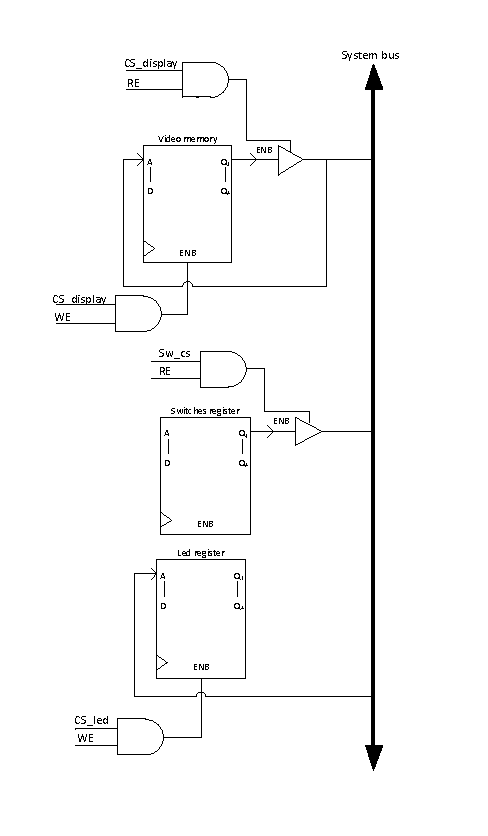
\epsfig{file=fig/system.eps, width=3.0in}
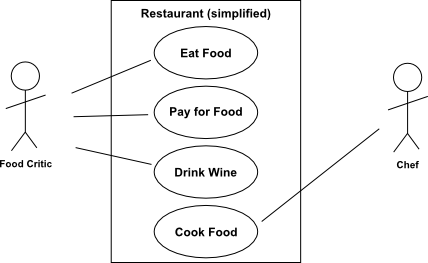
\includegraphics[scale=0.6]{fig/UML_Use_Case_diagram.png} 
\caption{Use Case Diagram example}
\label{fig:use_case_diagram_example}
\end{figure}

\subsection{State diagrams}
\begin{figure}[h]
\centering
%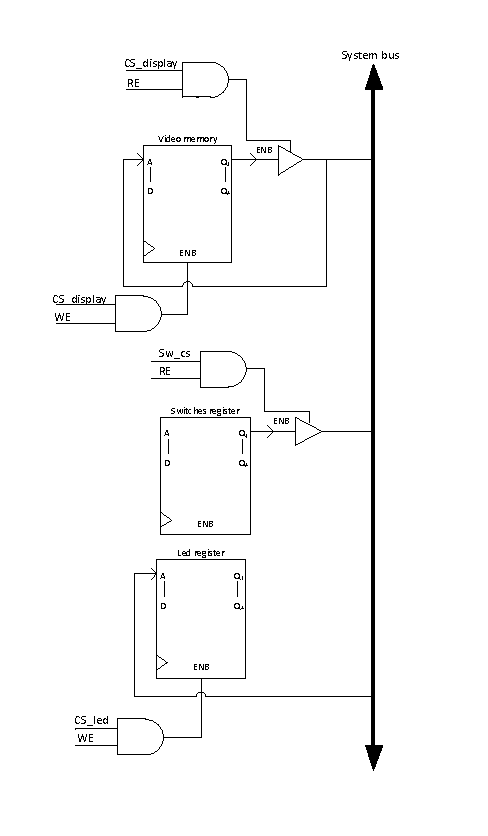
\epsfig{file=fig/system.eps, width=3.0in}
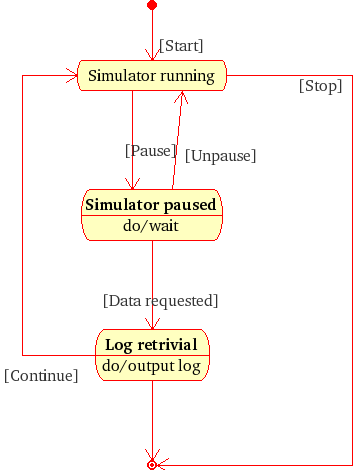
\includegraphics[scale=0.45]{fig/UML_state_diagram.png} 
\caption{State Diagram example}
\label{fig:state_diagram_example}
\end{figure}

The state diagram is also widely used in digital electronics.


\subsubsection{Sequence diagrams}

\subsubsection{Other types}


\subsubsection*{Flow diagrams}
Though strictly not a part of UML, classic flow diagrams are a good addition to use case diagrams.


\subsection{Discussion}
The main advantage of UML is primarily found in the software engineering field - and from this perspective. However, it has proved itself to be a very powerful communication tool, when work-flow and logic has to be modelled in software.

Applying some of the techniques to other engineering disciplines can, potentially, provide benefits - but is also liable to the common pitfalls of trying using tool in a way it was not intended to be used.

UML is subject to continuous critique from the software engineering field, and these points should be taken into consideration in an adoption.

\section{Software Project management}
A lot of time, work and money can be saved if an existing software management tool is converted to a specialized EN-50126 tool.

This section is meant as a brief description of some of the existing tools available.
\subsection{Bugzilla}
Bugzilla has been around since the 

\subsection{Tracks}
Tracks implement the Getting Things Done methodology\footnote{TODO}. Which is a simplistic approach to put a system to relatively sporadic ideas and tasks continuously. It is also project oriented, but is more dynamic in nature.

\subsection{Redmine}
Redmine is a more full-featured project management tool.


\end{document}